\section*{Oscilador libre de un único grado de libertad}

\item 
\begin{minipage}[t][6.2cm]{0.7\textwidth}
\textbf{Péndulo ideal}\\
Un péndulo de longitud $l$ está sometido a la aceleración gravitatoria \(\vec{g}\).
\begin{enumerate}
	\item Discuta todas las aproximaciones que realiza para arribar al modelo de "péndulo ideal", y para su dinámica en "pequeñas oscilaciones".
	\item Escriba y resuelva las ecuaciones de movimiento 
	\item (*) Grafique la tensión del hilo en función del ángulo para pequeñas oscilaciones de un péndulo ideal.
	En particular piense cómo afecta esta tensión la validez de la hipótesis de longitud de hilo constante.
	Dé valores de orden de magnitud razonables a los parámetros que necesite para la discusión.
	¿Es razonable la aproximación g = constante?
\end{enumerate}
\end{minipage}
\begin{minipage}[c][0cm][t]{0.25\textwidth}
	% 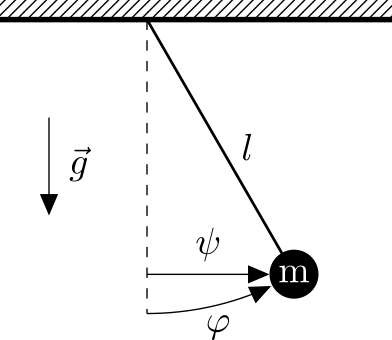
\includegraphics[width=\textwidth]{penduloHorizontal}
	\begin{tikzpicture}[scale= 1.2]
	% \begin{tikzpicture}
  	\draw [arrows=- triangle 45] (-1,2) -> (-1,1) node [above=15, right=2] {\(\vec{g}\)}; % g vertical
		\draw [ultra thick] (-1.5,3) -- (2.5,3);
		\fill [pattern = north east lines] (-1.5,3) rectangle (2.5,3.2); % techo
		\draw [dashed] (0,3) -- (0,0);	% vertical
		\draw [thick] (0,3) -- +(-60:3) node[midway,above,right=2] {\(l\)};	% inclinada +:relativa, -60 grados, longitud 3
		% \draw [thick] (0,3) -- +(-60:3) node[midway,above,sloped] {\(l\)};	% inclinada +:relativa, -60 grados, longitud 3
    \fill (0,3)+(-60:3) circle [radius=0.25] node [text=white] { \( \mathrm{m} \) }; % masa izq
    \draw [thin, arrows=- triangle 45] (0,.4) -> (1.25,.4) node [midway, above] {\( \psi \)}; % desplazamiento horizontal
    % \draw [thin, arrows=- triangle 45] (0,.4) -> (1.25,.4) node [above=8, left=8] {\( \psi \)}; % desplazamiento horizontal
		\draw [thin, arrows=- triangle 45] (0,0) arc [start angle=-90, end angle=-65, radius=3] node [below=12, left=8] {\( \varphi \)};
	\end{tikzpicture}
\end{minipage}



\item
\begin{minipage}[t][1.9cm]{0.7\textwidth}
\textbf{Resortes antagónicos}\\
El sistema de la figura muestra un peso, de masa $m$, suspendido equidistante de dos paredes por dos resortes antagónicos de idéntica constante elástica $k$, y longitud en el reposo $l$.
Se asume que no hay aceleración gravitatoria $\vec{g}$.
\end{minipage}
\begin{minipage}[c][0cm][t]{0.25\textwidth}
  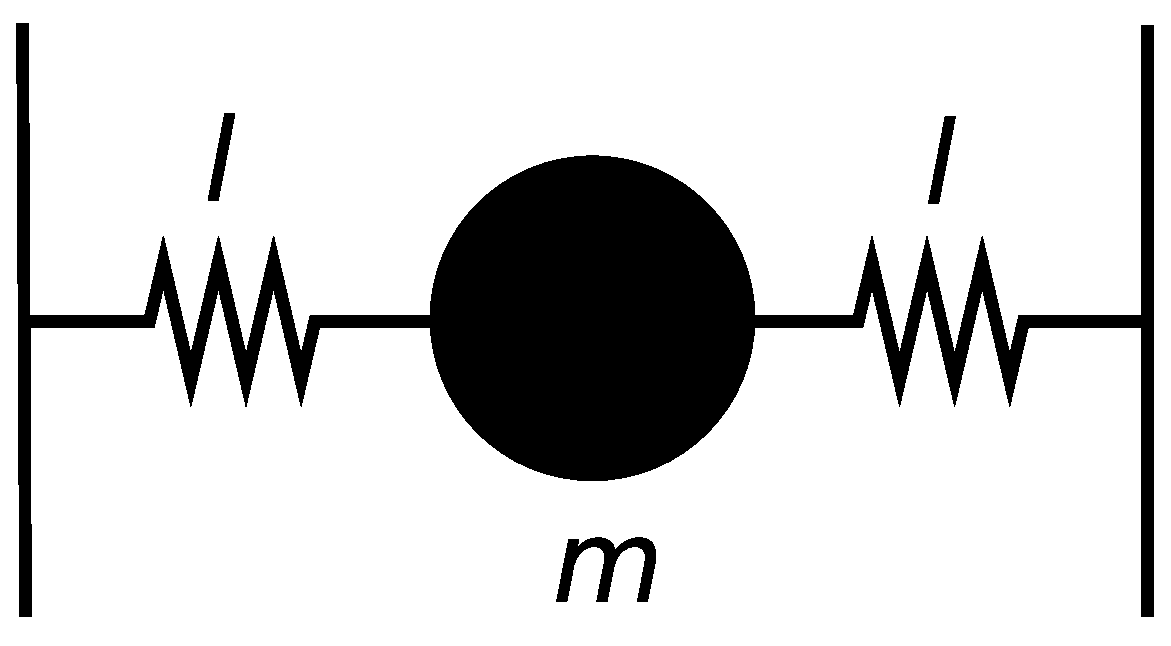
\includegraphics[width=\textwidth]{ej1-1}
\end{minipage}
\begin{enumerate}
	\item Analice las oscilaciones longitudinales para los casos:   
	\begin{enumerate}
		\item longitud natural del resorte $l_0$ ($l_0 < l$),   
		\item resortes muy elongables o ``slinkies'' ($l_0 = 0$).   
	\end{enumerate}
	\item Analice las oscilaciones transversales del sistema, discutiendo las diferencias entre los casos 1) y 2), y analizando cuidadosamente las aproximaciones que realiza.
	En el caso 1) analice la diferencia entre considerar que los resortes están tensionados en la posición de equilibrio $(l_{0}<l)$ y el coso en que están relajados en dicha posición $(l_0= l)$.
\end{enumerate}



\item 
\textbf{Resorte colgante}\\
Resuelva la dinámica para un peso colgado de un resorte vertical que pende de un techo.
Use como origen de la coordenada relevante cero la posición del resorte en reposo sin peso.
Escriba la energía potencial (gravitatoria + elástica) y encuentre la posición de equilibrio.
Al oscilar, ¿la energía potencial es solo la del resorte o también ``oscila'' la potencial gravitatoria?
